% ==================================================================
\section{问题二：局部模态缺失下的情感预测}\label{sec:q2}
% ==================================================================

问题二在附件2的50位置特征上，同时预测片段的三分类极性和连续强度，并衡量局部连续缺失对两类输出的影响。本章先说明三种掩码怎么分开，再给出正式模型 PM-B2 和评估面板，然后依次报告基线比较、缺失规律、测试集误差分析和我们做过的改进尝试，最后对附件3推理。

\subsection{数据、标签与三种掩码}\label{sec:q2data}

每条样本在同一条50位置轴上给出文本、声学、视觉矩阵，维度分别为 $50\times768$、$50\times74$、$50\times35$。情感强度 $y_i\in[-3,3]$；类别由原标注固定为负向、中性、正向三类，编码为0、1、2，其中 $y_i=0$ 只属于中性。训练只用训练集的标签，验证集用于选结构、超参数和检查点。

矩阵里的零可能来自补齐填充、原生不可观测或我们施加的遮蔽，因此对样本 $i$、模态 $m$、位置 $t$ 分别记录布局掩码 $\ell_{imt}$、原生可观测掩码 $o_{imt}$ 和人为遮蔽掩码 $s_{imt}$。实际送入模型的是
\begin{equation}\label{eq:mask}
a_{imt}=o_{imt}(1-s_{imt}),\qquad \tilde{\boldsymbol x}_{imt}=a_{imt}\,\frac{\boldsymbol x_{imt}-\boldsymbol\mu_m}{\boldsymbol\sigma_m},
\end{equation}
其中 $\boldsymbol\mu_m$、$\boldsymbol\sigma_m$ 只用训练集中可观测位置估计，标准化以后再把不可观测位置清零。文本掩码排除 \texttt{[CLS]}、\texttt{[SEP]} 和补齐位，声学、视觉掩码由非零行确定。布局掩码 $\ell$ 保留原来的位置范围：序列内部的缺口仍占着原来的序号，不会被挤到序列末尾。三种模态全部不可用时，模型直接返回训练集的类别频率和强度中位数，避免从一个空输入里得出针对具体样本的结论。

\subsection{PM-B2 池化双头模型}\label{sec:pmb2}

模型的思路很朴素：先把每个模态的可观测位置汇总成固定长度的统计量，再用一个小网络同时预测类别和强度。对模态 $m$，在可用位置上求均值和标准差：
\begin{equation}\label{eq:pool2}
\boldsymbol\mu_{im}=\frac{\sum_t a_{imt}\tilde{\boldsymbol x}_{imt}}{\max\!\big(1,\sum_t a_{imt}\big)},\qquad
\boldsymbol d_{im}=\left[\boldsymbol\mu_{im},\ \sqrt{\frac{\sum_t a_{imt}\big(\tilde{\boldsymbol x}_{imt}-\boldsymbol\mu_{im}\big)^{\odot2}}{\max\!\big(1,\sum_t a_{imt}\big)}}\ \right],
\end{equation}
可用位置为空时两项都取零向量。这种池化天然适应缺失：缺了一段，只是参与平均的位置少了，不会像序列模型那样在缺口处读到一串假的零。

三路拼接后的维度为 $2\times(768+74+35)=1754$。PM-B2 用 $1754\to128\to64$ 的两层 ReLU 网络融合，层间 dropout 为0.2；64维共享表示后面接两个独立的线性头，一个输出三类 logits $\boldsymbol z_i$，一个输出强度原值 $u_i$：
\begin{equation}\label{eq:heads}
\begin{gathered}
\boldsymbol p_i=\mathrm{softmax}(\boldsymbol z_i),\qquad \hat c_i=\mathop{\arg\max}_{c\in\{0,1,2\}}p_{ic},\qquad
\hat y_i=3\tanh(u_i),\\
\mathcal{L}=\frac{1}{B}\sum_{i=1}^{B}\Big[-\log p_{i,c_i}+\big|y_i-\hat y_i\big|\Big].
\end{gathered}
\end{equation}
$3\tanh$ 把强度限制在 $[-3,3]$ 内，回归用 L1 损失，与评价指标 MAE 一致。两个输出来自同一个检查点，但分类结果并不由强度的正负号决定，所以会出现“判为中性、强度略偏正”这样的组合，这是两个头各自判断的结果，并非拼接错误。训练设置见表\ref{tab:q2train}。

\begin{table}[htbp]
\centering
\caption{PM-B2 的训练设置}
\label{tab:q2train}
\begin{tabularx}{\textwidth}{l>{\raggedright\arraybackslash}X}
\toprule
项目 & 设置 \\
\midrule
数据 & 附件2 aligned\_50：训练集3395条拟合，验证集728条选型 \\
网络 & 均值+标准差池化 $\to$ 1754 $\to$ 128 $\to$ 64（ReLU，dropout 0.2）$\to$ 分类头 + 强度头 \\
优化 & AdamW，学习率 $3\times10^{-4}$，批大小64，最多30轮 \\
随机种子 & 17、29、43 用于结构比较；专项推理部署 seed 17 \\
检查点选择 & 验证集63档平均 macro-F1 优先，63档平均 MAE 其次，同分取较早轮次 \\
训练遮蔽 & PM-B2 本身不做训练遮蔽；对照模型的缺失增广用固定种子 20260923 生成的双窗口库 \\
复现 & 参数、代码与输入缓存的哈希写入冻结清单 \\
\bottomrule
\end{tabularx}
\end{table}

\subsection{局部缺失面板与评价指标}\label{sec:panel}

正式面板 $\mathcal{K}_{PM}$ 只在被选中的模态里删除一段连续窗口，其余模态保持原样。设某模态原可观测位置的首、尾序号为 $f$、$l$，跨度 $L=l-f+1$。对名义缺失比例 $r\in\{0.1,0.3,0.5\}$，窗口宽度取 $\max(1,\lfloor rL\rfloor)$，起点取头、中、尾三者之一，截出的区间再与 $o_{imt}$ 取交。可观测位置少于两个时不删除，并保证不会把原本可观测的模态整个删空。由于原生缺口、特殊词元和取整的存在，实际删除比例
\begin{equation}\label{eq:rho}
\rho_{im}=\frac{\sum_t o_{imt}s_{imt}}{\max\!\big(1,\sum_t o_{imt}\big)}
\end{equation}
未必等于名义比例，所以后文的10\%、30\%、50\%指的是名义档位。文本的遮蔽不是简单地把缓存的 BERT 向量置零，而是从原始词元输入里移除相应位置，再经同一个冻结的 BERT 重新编码，这样被删掉的词也不会通过上下文“泄漏”到其他位置。验证时统一使用确定的头、中、尾窗口。

被遮蔽模态的非空组合有 $T$、$A$、$V$、$TA$、$TV$、$AV$、$TAV$ 七种，与3种比例、3种位置组合成 $7\times3\times3=63$ 档。每一档都在同一批728条验证样本上计算指标，再对63档等权平均。评价指标为
\begin{equation}\label{eq:metrics}
\begin{gathered}
\mathrm{Acc}=\frac{1}{n}\sum_i\mathbb{1}(\hat c_i=c_i),\qquad
F_{1,\mathrm{macro}}=\frac{1}{3}\sum_{c=0}^{2}\frac{2P_cR_c}{P_c+R_c},\\
\mathrm{MAE}=\frac{1}{n}\sum_i|\hat y_i-y_i|,\qquad
\bar F_{1,63}=\frac{1}{63}\sum_{k=1}^{63}F_{1,k},
\end{gathered}
\end{equation}
其中 $P_c$、$R_c$ 为第 $c$ 类的精确率和召回率，分母为零时该类 F1 记为0；$\overline{\mathrm{MAE}}_{63}$ 同样先逐档再平均。皮尔逊相关系数在预测或真实强度为常数时记为未定义，而不是记为0。

\subsection{基线比较与缺失训练消融}\label{sec:baseline}

表\ref{tab:baselines}列出了在同一正式面板上比较的7个基线：B0 直接输出训练集先验；B1-T、B1-A、B1-V 是单模态池化线性模型；B3 对三个单模态输出做固定权重的决策融合；B1-N 是文本双向 LSTM；B4 是低秩融合\cite{liu2018lmf}。图\ref{fig:baselines}把它们画在同一张图上。

\begin{table}[htbp]
\centering
\caption{正式局部缺失面板上的结构比较（验证集728条、63档；神经网络模型为 seed 17/29/43 的均值 $\pm$ 标准差）}
\label{tab:baselines}
\begin{tabular}{lcc}
\toprule
模型 & 63档平均 macro-F1 & 63档平均 MAE \\
\midrule
B0 训练集先验 & 0.2114 & 0.7690 \\
B1-T 单文本 & 0.4979 & 0.9095 \\
B1-A 单声学 & 0.3526 & 0.8263 \\
B1-V 单视觉 & 0.3455 & 0.7818 \\
B3 决策融合 & 0.4983 & 0.7277 \\
B1-N 文本 BiLSTM & 0.5520 $\pm$ 0.0090 & 0.6523 $\pm$ 0.0144 \\
B4 低秩融合 & 0.5686 $\pm$ 0.0057 & 0.6248 $\pm$ 0.0079 \\
PM-B2 池化双头 & \textbf{0.5752 $\pm$ 0.0013} & \textbf{0.6213 $\pm$ 0.0123} \\
\bottomrule
\end{tabular}
\end{table}

\begin{figure}[htbp]
\centering
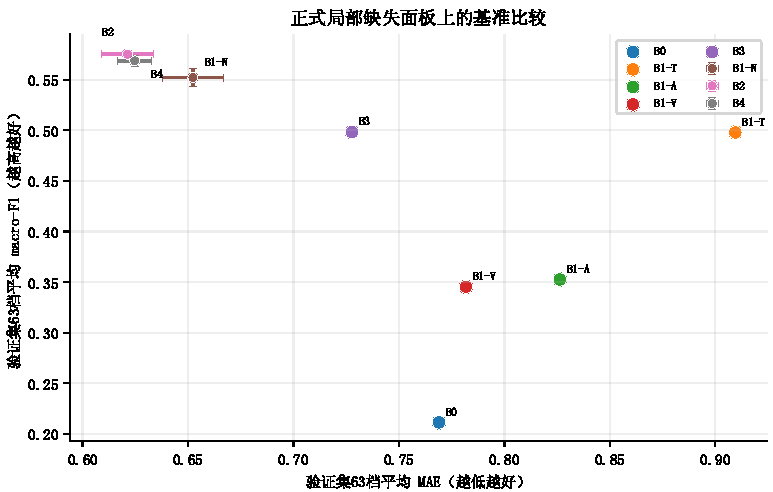
\includegraphics[width=0.8\textwidth]{figures/fig_q2_baselines.pdf}
\caption{各基线在正式面板上的表现（横轴63档平均 MAE，越左越好；纵轴63档平均 macro-F1，越高越好；B1-N、B2、B4 的误差线为三个种子间的标准差，图中 B2 即 PM-B2）}
\label{fig:baselines}
\end{figure}

PM-B2 在 F1 和 MAE 上都是7个模型里最好的，而且三个种子间的 F1 标准差只有0.0013，远小于 B1-N 和 B4。几个单模态基线也很说明问题：只用文本的 B1-T 的 F1 接近0.50，只用声学或视觉的都在0.35左右，只比先验好一截。B0 的 F1 只有0.2114，比三分类随机的1/3还低，因为它永远预测多数类，另外两类的 F1 都是0。

参数更多的时序模型是否值得？我们在同样的学习率和三个种子下做了一个 $2\times2$ 消融：M0 是不做缺失增广、也不显式使用可观测掩码的跨模态时序网络；M1 只加连续遮蔽训练；M2 只让注意力和池化显式使用可观测掩码；M3 两者都用。结果见表\ref{tab:m0m3}。

\begin{table}[htbp]
\centering
\caption{跨模态时序模型的 $2\times2$ 消融（验证集728条、正式面板63档、三种子均值）}
\label{tab:m0m3}
\begin{tabular}{ccccc}
\toprule
配置 & 训练遮蔽 & 显式可观测掩码 & macro-F1 & MAE \\
\midrule
M0 & 否 & 否 & 0.5555 & 0.6295 \\
M1 & 是 & 否 & 0.5630 & 0.6290 \\
M2 & 否 & 是 & 0.5648 & 0.6273 \\
M3 & 是 & 是 & 0.5682 & 0.6195 \\
\bottomrule
\end{tabular}
\end{table}

两个因素各自都有一点帮助，合在一起的 M3 比 M0 的 F1 高0.0127、MAE 低约0.010；按源视频做配对重抽样，F1 差的95\%区间为 $[0.0049,0.0214]$，不跨零。但即便是 M3，F1 也还是比 PM-B2 低0.007；M3 的 MAE（0.6195）比 PM-B2 略低0.0018，这点差距远小于 PM-B2 自身0.0123的种子间波动。在本题的数据量下，更复杂的时序结构没有换来明显的收益，这也是我们最终选 PM-B2 作为正式模型的原因。

\subsection{缺失类型、比例与位置的影响}\label{sec:law}

表\ref{tab:law}按被遮蔽模态、名义比例和位置三个因素，把部署模型（seed 17）在验证集和测试集上的63档结果分组平均；图\ref{fig:law}是对应的图。每个模态组合跨9档平均，每个比例或位置跨21档平均。

\begin{table}[htbp]
\centering
\caption{PM-B2（seed 17）在正式面板上的分组结果}
\label{tab:law}
\begin{tabular}{llcccc}
\toprule
因素 & 档位 & 验证集 F1 & 验证集 MAE & 测试集 F1 & 测试集 MAE \\
\midrule
\multirow{7}{*}{被遮蔽模态} & $T$ & 0.5563 & 0.6487 & 0.5894 & 0.6979 \\
 & $A$ & 0.5975 & 0.6125 & 0.6144 & 0.6500 \\
 & $V$ & 0.5942 & 0.6126 & 0.6156 & 0.6494 \\
 & $TA$ & 0.5583 & 0.6494 & 0.5887 & 0.6985 \\
 & $TV$ & 0.5573 & 0.6488 & 0.5900 & 0.6988 \\
 & $AV$ & 0.5952 & 0.6131 & 0.6162 & 0.6507 \\
 & $TAV$ & 0.5582 & 0.6495 & 0.5908 & 0.6994 \\
\midrule
\multirow{3}{*}{名义比例} & 10\% & 0.5905 & 0.6180 & 0.6141 & 0.6601 \\
 & 30\% & 0.5716 & 0.6300 & 0.6001 & 0.6756 \\
 & 50\% & 0.5595 & 0.6526 & 0.5879 & 0.6978 \\
\midrule
\multirow{3}{*}{位置} & 头 & 0.5761 & 0.6397 & 0.6002 & 0.6778 \\
 & 中 & 0.5734 & 0.6283 & 0.6072 & 0.6678 \\
 & 尾 & 0.5720 & 0.6326 & 0.5948 & 0.6879 \\
\bottomrule
\end{tabular}
\end{table}

\begin{figure}[htbp]
\centering
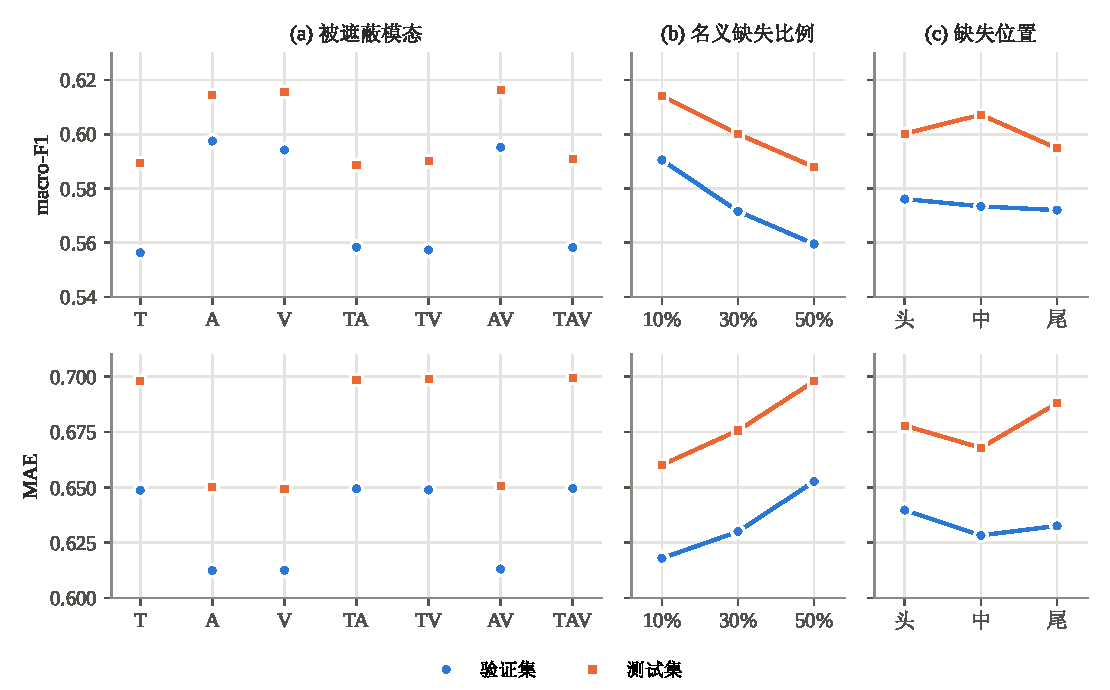
\includegraphics[width=\textwidth]{figures/fig_q2_missing_law.pdf}
\caption{缺失类型、比例与位置对 macro-F1（上）和 MAE（下）的影响（数据同表\ref{tab:law}；模态组合是无序类别，不连线）}
\label{fig:law}
\end{figure}

三个因素的作用大小差别很明显。

\textbf{模态类型影响最大，而且只看“有没有遮文本”。}七种组合清楚地分成两组：凡是遮蔽了文本的（$T$、$TA$、$TV$、$TAV$），验证集 F1 都在0.556～0.558之间；只遮蔽声学或视觉的（$A$、$V$、$AV$），都在0.594～0.598之间，两组相差约0.04，MAE 相差约0.036。组内几乎没有差别，比如在遮蔽文本的基础上再遮蔽声学和视觉（$TAV$），与只遮蔽文本（$T$）相比 F1 几乎不变。这说明当前模型的判断主要依赖文本，声学和视觉局部缺一段对它影响很小。但这不等于声学、视觉在所有样本上都没有用，第\ref{sec:q3}章的逐样本归因会看到少数样本主要依靠它们。

\textbf{缺失比例的影响是单调的。}名义比例从10\%增至50\%，验证集 F1 由0.5905降到0.5595，MAE 由0.6180升到0.6526；测试集的走势完全一致。

\textbf{位置的影响最小，且不稳定。}验证集上头、中、尾的 F1 最大相差0.0041，测试集上相差0.0124，而且两个集合上的排序不一样：验证集是头最好，测试集是中间最好。所以我们不认为存在某个“普遍最要紧”的时间位置。

\subsection{完整输入的结果与错误归因}\label{sec:q2err}

表\ref{tab:q2full}汇总了 PM-B2 在完整输入下的结果。三种子平均、单个部署权重、不同输入条件是三个不同的统计对象，表中分开列出。

\begin{table}[htbp]
\centering
\caption{PM-B2 的完整输入结果}
\label{tab:q2full}
\begin{tabular}{llcccc}
\toprule
对象 & 输入 & Acc & macro-F1 & MAE & Pearson \\
\midrule
验证集三种子均值 & 完整 & 0.6264 & 0.5988$\pm$0.0033 & 0.5998$\pm$0.0128 & -- \\
验证集 seed 17 & 完整 & 0.6277 & 0.6002 & 0.6120 & -- \\
验证集 seed 17 & 63档平均 & -- & 0.5739 & 0.6335 & -- \\
测试集 seed 17 & 完整 & 0.6644 & 0.6147 & 0.6485 & 0.6691 \\
测试集 seed 17 & 63档平均 & -- & 0.6007 & 0.6778 & -- \\
\bottomrule
\end{tabular}
\end{table}

测试集完整输入的混淆矩阵（行为真实的负、中、正，列为预测的负、中、正）及由它算出的各类指标见表\ref{tab:cm}。

\begin{table}[htbp]
\centering
\caption{测试集（727条）完整输入的混淆矩阵与分类指标}
\label{tab:cm}
\begin{tabular}{l|ccc|c|ccc}
\toprule
真实 $\backslash$ 预测 & 负 & 中 & 正 & 合计 & 精确率 & 召回率 & F1 \\
\midrule
负 & \textbf{156} & 23 & 28 & 207 & 0.645 & 0.754 & 0.695 \\
中 & 43 & \textbf{57} & 58 & 158 & 0.442 & 0.361 & 0.397 \\
正 & 43 & 49 & \textbf{270} & 362 & 0.758 & 0.746 & 0.752 \\
\midrule
合计 & 242 & 129 & 356 & 727 & \multicolumn{3}{c}{macro-F1 $=0.6147$} \\
\bottomrule
\end{tabular}
\end{table}

我们按这张表和前面的结果，把错误归纳为以下几类。

\textbf{（1）中性类是主要短板。}负向和正向的召回都在0.75左右，中性只有0.361，F1 只有0.397，拉低了整体的 macro-F1。158条真实中性里，58条被判为正向、43条被判为负向，判对的只有57条。反过来，模型判为中性的129条里也只有57条是对的。换句话说，模型并不是分不清任意两类，而是分不清“中性”和“轻微的正、负”。考虑到中性只对应 $y=0$ 这一个值，而标注是多人评分的平均，“略偏正”和“中性”的边界本身就不清晰，这个问题并不意外。

\textbf{（2）正、负之间也有互相误判。}负向被判为正向的有28条，正向被判为负向的有43条，合计71条，比负、中之间的互相误判（66条）还略多。这部分可能与反讽、转折类句子有关，但仅凭预测与标签的统计，我们不能断定是哪一类语言现象造成的。

\textbf{（3）测试集上强度误差偏大。}测试集完整输入的 MAE（0.6485）高于验证集（0.6120），说明冻结的权重在测试集上的强度误差有所上升，而分类指标反而更好。两者方向不一致，提示强度尺度的校准可能需要单独处理。

\textbf{（4）对文本的依赖过重。}第\ref{sec:law}节的分组结果显示，遮蔽文本是性能下降的主要来源。转写一旦出错，模型很难靠声学和视觉补回来。

\subsection{改进尝试：A–E 五阶段开发实验}\label{sec:ae}

PM-B2 冻结并完成附件3推理以后，我们又只用训练集和验证集、固定 seed 17，做了五个阶段共15种配置的改进尝试，想看看能否在完整输入和缺失两方面同时做得更好。这些实验没有读取测试集和附件3、4。先说结论：完整输入的 F1 确实能提高，但换来的是在更严格的缺失条件下明显退化，没有一个配置在各项指标上全面超过 PM-B2 这条主线，所以正式结果仍以 PM-B2 为准。

\subsubsection{更严格的整模态保留面板}

为了检验这些模型在更极端条件下的表现，我们另设了一个压力面板 $\mathcal{K}_{LH}$：先选一个保留的模态子集 $S\in\{T,A,V,TA,TV,AV,TAV\}$，把 $S$ 以外的模态整路关闭，再只在 $S$ 内施加10\%、30\%、50\%和头、中、尾的连续窗口。它同样是 $7\times3\times3=63$ 档，但含有整路缺失的压力，比正式面板苛刻得多。两个面板的输入分布不同，数值不能互相比较；例如 PM-B2 在正式面板上的0.5752和下面层次头模型在压力面板上的0.4139，并不说明前者“好了0.16”。

\subsubsection{A–C 阶段：文本适配、中性判别与音视频补充}

A 阶段在附件2训练集上用 LoRA\cite{hu2022lora}适配文本表示：在冻结的 BERT 权重 $W_0$ 上学习低秩增量，即 $W=W_0+(\alpha/r)BA$，取秩8、$\alpha=16$、适配器 dropout 0.05。由于要在线更新文本表示，这一阶段直接用原始 text\_bert 的词元编号、注意力掩码和分段输入，而不用原来的 BERT 缓存。我们固定六个组合（冻结或 LoRA、文本单路或三模态、两种学习率），结果见表\ref{tab:stageA}。

\begin{table}[htbp]
\centering
\caption{A 阶段完整输入的验证集结果（728条，seed 17，各取 F1 最优检查点）}
\label{tab:stageA}
\begin{tabular}{lccc}
\toprule
配置 & Accuracy & macro-F1 & MAE \\
\midrule
冻结，文本 & 0.6415 & 0.6036 & 0.5984 \\
冻结，三模态（修复后重训） & 0.6346 & 0.5959 & 0.5953 \\
LoRA，文本，$10^{-4}$ & 0.6538 & 0.6152 & 0.6008 \\
LoRA，三模态，$10^{-4}$（修复后重训） & 0.6442 & 0.6054 & 0.5854 \\
LoRA，文本，$3\times10^{-4}$ & 0.6525 & 0.6052 & 0.5592 \\
LoRA，三模态，$3\times10^{-4}$（修复后重训） & 0.6442 & 0.6203 & 0.5945 \\
\bottomrule
\end{tabular}
\end{table}

LoRA 组整体好于冻结组，F1 最高的是三模态、学习率 $3\times10^{-4}$ 的0.6203。不过这只是单种子的结果，而且冻结组和适配组的训练过程本身也不同，我们不把增益全部归功于 LoRA。表中标注“修复后重训”的三行，是在发现评估代码的问题（见第\ref{sec:fix}节）后重新训练得到的。

B 阶段针对中性类，从 A 阶段的文本 LoRA 模型（学习率 $10^{-4}$）继续训练，试了两条路。B1 按训练集各类样本数 $(967,758,1670)$ 的平方根倒数给分类交叉熵加权。B2 改用层次输出：令 $q=P(\text{中性})$，$r=P(\text{正向}\mid\text{非中性})$，三类概率为
\begin{equation}\label{eq:hier}
(p_{\mathrm{neg}},p_{\mathrm{neu}},p_{\mathrm{pos}})=\big((1-q)(1-r),\ q,\ (1-q)r\big),
\end{equation}
分类损失为中性的二元交叉熵，加上非中性样本的正向二元交叉熵，推理时仍取概率最大的一类。我们把 B2 得到的模型记为 LH-B2，它和 PM-B2 不是同一个模型。两条路都提高了中性召回（由0.337分别升到0.495和0.429），但中性精确率也由0.508降到0.455和0.473，没能同时改善。LH-B2 的完整输入 F1 为0.6244，是各阶段中最高的，因此作为后续 C、D、E 阶段的基础模型。

C 阶段尝试两种音视频补充方式：C1 在 BERT 中间层注入局部音视频残差，C2 在池化特征上分别为分类和回归学习门控。结果见表\ref{tab:stageBC}：C1 的 F1 和 MAE 都不如基础模型；C2 的回归误差下降了，分类却退步。两者都没有形成全面优势，后续没有并入主线。

\begin{table}[htbp]
\centering
\caption{B、C 阶段完整输入的验证集结果（728条，seed 17）}
\label{tab:stageBC}
\begin{tabular}{lcccc}
\toprule
检查点 & Accuracy & macro-F1 & MAE & 中性 F1 \\
\midrule
A 阶段文本模型（B 阶段起点） & 0.6566 & 0.6143 & 0.5877 & 0.4052 \\
B1 加权分类 & 0.6429 & 0.6217 & 0.5692 & 0.4740 \\
B2 层次头（LH-B2） & 0.6484 & \textbf{0.6244} & 0.5987 & 0.4501 \\
C1 局部注入（修复后重训） & 0.6374 & 0.5910 & 0.6225 & 0.3576 \\
C2 两任务独立门控 & 0.6264 & 0.6069 & 0.5857 & 0.4309 \\
\bottomrule
\end{tabular}
\end{table}

\subsubsection{D–E 阶段：表征分解、缺失增广与蒸馏}

D 阶段固定 LH-B2 的文本适配器。D1 只训练小型残差任务头和一个监督对比投影\cite{khosla2020supcon}，正例要求同类且来自不同源视频；D2 借鉴共享/私有表示的思路\cite{hazarika2020misa}，把三模态池化表示拆成共享和私有两支，加上共享对齐、共享与私有的协方差约束和输入重建三个辅助项。E 阶段以 D2 为学生、LH-B2 为固定教师：E0 继续训练但不做缺失增广；E1 在一半样本上按预定的模态组合、比例和窗口合成缺失；E2 在 E1 的基础上再加入对教师分类分布的温度 KL、强度 L1 和批内关系保持项。完整输入与压力面板的结果见表\ref{tab:stageDE}和图\ref{fig:shift}。

\begin{table}[htbp]
\centering
\caption{D、E 阶段在完整输入与整模态保留压力面板上的结果（验证集728条，seed 17；压力面板为63档等权平均）}
\label{tab:stageDE}
\begin{tabular}{lccccc}
\toprule
模型 & 完整 Acc & 完整 F1 & 完整 MAE & 压力 F1 & 压力 MAE \\
\midrule
LH-B2（基础） & 0.6484 & 0.6244 & 0.5987 & 0.4139 & 0.6977 \\
D1 对比头 & 0.6360 & 0.6005 & 0.5912 & 0.4110 & 0.6937 \\
D2 共享/私有 & 0.6401 & 0.6176 & 0.5791 & 0.4286 & 0.7556 \\
E0 无增广 & 0.6113 & 0.5739 & 0.5815 & 0.4500 & 0.7450 \\
E1 缺失增广 & 0.6154 & 0.5578 & 0.5832 & 0.4512 & 0.7279 \\
E2 增广+蒸馏 & 0.6223 & 0.5742 & 0.5891 & 0.4518 & 0.7423 \\
\bottomrule
\end{tabular}
\end{table}

\begin{figure}[htbp]
\centering
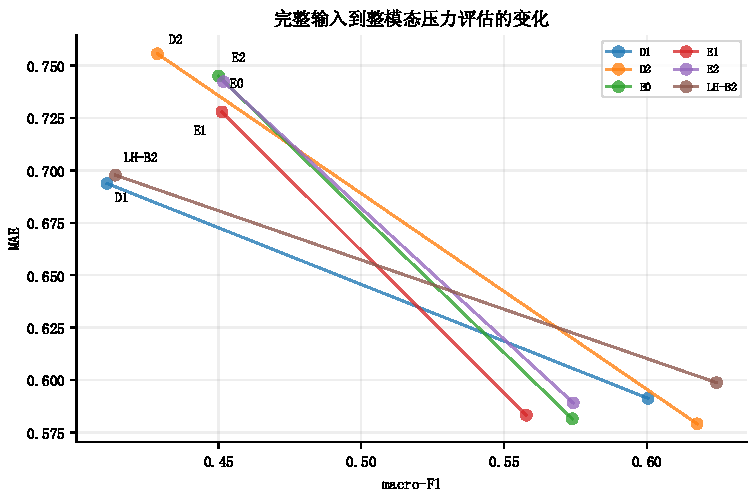
\includegraphics[width=0.78\textwidth]{figures/fig_q2_lh_shift.pdf}
\caption{各检查点从完整输入（右下端点）到压力面板（左上端点）的变化；横轴 macro-F1 越大越好，纵轴 MAE 越小越好}
\label{fig:shift}
\end{figure}

图\ref{fig:shift}里的每条线都从右下往左上走，而且完整输入越好的模型，压力面板上往往越差：LH-B2 的完整输入 F1 最高（0.6244），压力面板 F1 却排在倒数第二（0.4139）；E 阶段三个模型正好相反，压力面板 F1 都在0.45左右（连不做增广的 E0 也是如此），完整输入 F1 却降到了0.56～0.57。再以 D2 为例，它的完整输入 MAE 比 LH-B2 低0.0196，压力面板 F1 高0.0147，可压力面板 MAE 却高了0.0579。

为了判断这些差异是不是抽样波动，我们按验证集的239个源视频做了1000次配对有放回抽样：每次对比较双方用相同的视频组频数，重算各档指标再平均，区间取2.5\%和97.5\%分位数。结果见表\ref{tab:boot}。

\begin{table}[htbp]
\centering
\caption{按源视频配对重抽样的差值（候选减参照；95\%区间，1000次）}
\label{tab:boot}
\begin{tabular}{llcc}
\toprule
比较 & 指标 & 点估计 & 95\%区间 \\
\midrule
\multirow{3}{*}{D2 $-$ LH-B2} & 完整 MAE & $-0.01965$ & $[-0.03470,\,-0.00379]$ \\
 & 压力 F1 & $+0.01469$ & $[+0.00134,\,+0.02738]$ \\
 & 压力 MAE & $+0.05793$ & $[+0.03261,\,+0.08086]$ \\
\midrule
\multirow{2}{*}{E1 $-$ E0} & 压力 F1 & $+0.00118$ & $[-0.01013,\,+0.01259]$ \\
 & 压力 MAE & $-0.01709$ & $[-0.02677,\,-0.00651]$ \\
\midrule
\multirow{2}{*}{E2 $-$ E1} & 压力 F1 & $+0.00056$ & $[-0.00886,\,+0.01117]$ \\
 & 压力 MAE & $+0.01440$ & $[+0.00631,\,+0.02243]$ \\
\bottomrule
\end{tabular}
\end{table}

D2 的三项差异区间都不跨零，说明它确实是用压力面板上的强度误差换来了完整输入的改善。E1 相对 E0 在压力面板上的 MAE 改善是可靠的，F1 的差异则跨零。E2 的蒸馏没有带来可靠的 F1 提升，MAE 反而变差。需要说明，验证集本身参与了检查点选择，这些实验也只有一个训练种子，所以上述区间描述的是已选模型在验证集视频抽样下的波动，不能当作独立测试集上的显著性结论。

\subsubsection{压力面板下的缺失诊断}

我们也在压力面板上看了 E2 的缺失规律。按保留的模态子集分组（表\ref{tab:e2group}），只保留声学或视觉时 F1 只有0.34和0.33左右，保留了文本的各组则在0.518～0.547之间。这再次说明，一旦文本整路不可用，模型就很脆弱。

\begin{table}[htbp]
\centering
\caption{E2 在压力面板上按保留模态分组的结果（每组9档，验证集728条）}
\label{tab:e2group}
\begin{tabular}{lcc@{\hspace{3em}}lcc}
\toprule
保留模态 & F1 & MAE & 保留模态 & F1 & MAE \\
\midrule
$T$ & 0.5179 & 0.7079 & $TA$ & 0.5259 & 0.6664 \\
$A$ & 0.3408 & 0.8805 & $TV$ & 0.5471 & 0.6377 \\
$V$ & 0.3256 & 0.8304 & $AV$ & 0.3623 & 0.8346 \\
$TAV$ & 0.5428 & 0.6388 & & & \\
\bottomrule
\end{tabular}
\end{table}

按名义比例汇总，10\%、30\%、50\%的 F1 依次为0.4623、0.4508、0.4421，MAE 依次为0.7227、0.7383、0.7659；按位置汇总，头、中、尾的 F1 为0.4509、0.4598、0.4446，MAE 为0.7431、0.7362、0.7477。比例的影响单调，位置的影响仍然较小，这与正式面板上的结论一致。这里的“时长”是50个位置上的比例，不能直接换算成秒数。

图\ref{fig:e2scan}把删除率加密扫描到0～1。在0～0.9之间，F1 随删除率缓慢下降、MAE 缓慢上升，删除率超过0.7以后变化明显加快。删除率为1.0时，保留子集里的所有模态都被删空，模型按规则退回训练集先验，F1 与 MAE 回到表\ref{tab:baselines}中 B0 的水平（0.2114和0.7690）。这一点是规则回退的结果，不是局部缺失曲线的自然延伸，图中单独看待。

\begin{figure}[htbp]
\centering
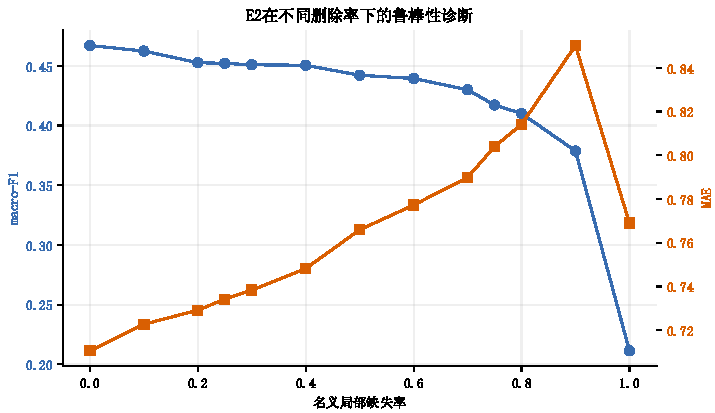
\includegraphics[width=0.78\textwidth]{figures/fig_q2_e2_scan.pdf}
\caption{E2 在不同名义删除率下的 macro-F1（蓝，左轴）与 MAE（橙，右轴），验证集728条，跨保留子集与位置平均}
\label{fig:e2scan}
\end{figure}

\subsubsection{评估代码的两处问题与修正}\label{sec:fix}

开发过程中我们发现评估代码有两处问题：一是不可用模态的数值仍然进入了预测路径；二是压力面板没有真正关闭保留子集以外的模态。受影响的是 A 阶段的三个三模态配置和 C1，它们都已按修正后的输入重新训练，D 阶段的面板也重新评估过；表\ref{tab:stageA}～表\ref{tab:stageDE}中的数值都是修正后的。

修正之后，我们给每次运行加了一道检查：对不可用模态施加任意数值扰动，预测变化必须小于 $10^{-6}$；全空输入必须返回训练集先验；重新加载权重后的预测必须一致。较早的 A、B、D 阶段是事后补做这项检查的，我们不把它们写成当时就已通过。这道检查本身不是新的预测算法，但它决定了上面这些数字能不能信。

\subsubsection{为什么没有替换正式模型}

15种配置里，完整输入 F1 最高的 LH-B2 比 PM-B2（三种子0.5988）高出约0.026，看起来值得替换。我们没有这样做，理由有三：第一，A–E 全部只跑了一个种子，胜出者还没有用 seed 29、43 复核；第二，这些模型在压力面板上普遍退化，说明完整输入的收益可能是以缺失下的稳健性为代价的，而问题二考的恰恰是缺失；第三，测试集已经看过一次，不能再用它来挑选模型。因此附件3的正式预测仍由 PM-B2 给出，A–E 的结果作为改进方向的依据写进论文。

\subsection{附件3推理}\label{sec:att3}

冻结的 PM-B2（seed 17）对附件3的30条样本全部完成了推理，逐条结果见附录\ref{app:B}的表\ref{tab:appB}，分布见图\ref{fig:special}(a)。

\begin{figure}[htbp]
\centering
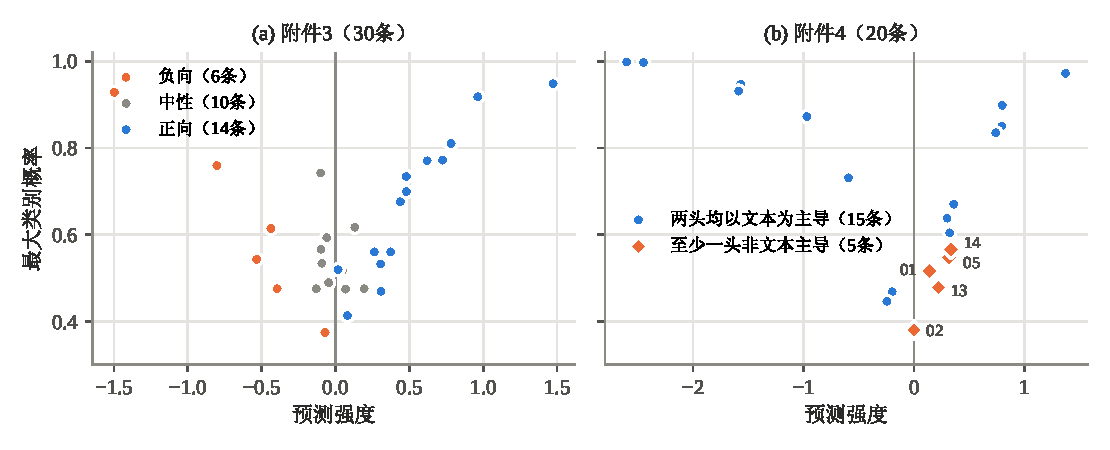
\includegraphics[width=\textwidth]{figures/fig_special_overview.pdf}
\caption{专项测试集的预测概览：(a) 附件3，按预测极性着色；(b) 附件4，按分类与强度两个输出的主导模态区分，橙色菱形为至少一个输出以非文本为主导的样本}
\label{fig:special}
\end{figure}

30条中正向14条、中性10条、负向6条，最大类别概率平均为0.619，其中8条低于0.5。极性与强度的正负号全部一致：判为正向的14条强度都为正（0.018～1.473），判为负向的6条都为负（$-1.497$～$-0.071$），判为中性的10条强度都落在 $[-0.130,0.194]$ 这一窄区间内。三类中中性的平均置信度最低（0.548，正向0.670、负向0.616），这与测试集上中性最难判断的结论是一致的。附件3没有标签，这些统计只能说明模型输出的内部一致性，不代表真实的情感分布或准确率。

\subsection{小结}

问题二的正式模型 PM-B2 结构很简单，却在7个基线和4个时序网络对照中取得了最高的缺失面板 F1，种子间波动也最小。缺失规律上，遮不遮文本是决定性因素，缺失比例的影响单调，位置的影响可以忽略。主要错误集中在中性类。A–E 改进尝试说明，完整输入的提升和缺失下的稳健性之间存在明显的取舍，在单种子证据下我们选择不替换正式模型。
